%\documentclass[preprint]{aastex}  % USE THIS TO MAKE BIB, THEN FORMAT USING EMULATEAPJ
\documentclass[onecolumn]{emulateapj} \shorttitle{}
\shortauthors{Ali, et al.}

\usepackage{amsmath} \usepackage{graphicx} \usepackage[figuresright]{rotating}
\usepackage{subfig}
%\usepackage{rotating}
\usepackage{natbib}
%\usepackage{pdflscape} \usepackage{lscape}
\citestyle{aa}

\def\b{\mathbf{b}} \def\k{\mathbf{k}} \def\r{\mathbf{r}} \def\q{\mathbf{q}}
\def\b{\mathbf{b}} \def\kp{\mathbf{k}^\prime}
\def\kpp{\mathbf{k}^{\prime\prime}} \def\V{\mathbb{V}} \def\expval#1{\langle #1
\rangle} \def\At{\tilde{A}} \def\Vt{\tilde{V}} \def\Tt{\tilde{T}}
\def\tb{\langle T_b\rangle} \newcommand{\vis}{\mathbf{v}}
\newcommand{\x}{\mathbf{x}} \newcommand{\xhat}{\hat{\mathbf{x}}}
\newcommand{\A}{\mathbf{A}} \newcommand{\N}{\mathbf{N}}
\newcommand{\C}{\mathbf{C}} \newcommand{\Q}{\mathbf{Q}}
\newcommand{\rhat}{\hat{\mathbf{r}}}
\newcommand{\phat}{\hat{\mathbf{p}}}
\newcommand{\qhat}{\hat{\mathbf{q}}}
\newcommand{\hMpci}{h\ {\rm Mpc}^{-1}}
\newcommand{\Tsys}{T_{\rm sys}}
\newcommand{\Tspin}{T_{\rm s}}
\newcommand{\kmin}{k_{\rm min}}
\newcommand{\kmax}{k_{\rm max}}
\newcommand{\Tcmb}{T_\gamma}
\newcommand\abs[1]{\left|#1\right|}
\newcommand{\mKlimit}{(22.4\,\textrm{mK})$^2$ }
\newcommand{\mKsqlimit}{503 mK$^2$}
\newcommand{\revisedmklimit}{(250\,\textrm{mK})^2}
\newcommand{\pobercitep}{(Pober et al. 2015, in prep)}
\newcommand{\pobercitet}{Pober et al. (2015, in prep)}
\newcommand{\parsonscitep}{(Parsons et al. 2015, in prep)}
\newcommand{\parsonscitet}{Parsons et al. (2015, in prep)}
\newcommand{\kolopaniscitet}{Kolopanis et al. (2018, submitted)}
\newcommand{\chengcitet}{\textrm{Cheng et al. (2018, submitted)}}


\begin{document}

\title{ERRATUM: ``PAPER-64 Constraints on Reionization: the  $21\,\textrm{cm}$ Power Spectrum at $z=8.4$" (2015, Apj, 809, 61)}

\author{
Zaki S. Ali\altaffilmark{1}, 
Aaron R. Parsons\altaffilmark{1,2}, 
Haoxuan Zheng\altaffilmark{3},
Jonathan C. Pober\altaffilmark{4}, 
Adrian Liu\altaffilmark{1,5}, 
James E. Aguirre\altaffilmark{6},
Richard F. Bradley\altaffilmark{7,8,9},
Gianni Bernardi\altaffilmark{10,11,12}, 
Chris L. Carilli\altaffilmark{13,14},
Carina Cheng\altaffilmark{1},
David R. DeBoer\altaffilmark{2}, 
Matthew R. Dexter\altaffilmark{2},
Jasper Grobbelaar\altaffilmark{10},
Jasper Horrell\altaffilmark{10},
Daniel C. Jacobs\altaffilmark{15}, 
Pat Klima\altaffilmark{8},
David H. E. MacMahon\altaffilmark{2},
Matthys Maree\altaffilmark{10},
David F. Moore\altaffilmark{6},
Nima Razavi\altaffilmark{14},
Irina I. Stefan\altaffilmark{14},
William P. Walbrugh\altaffilmark{10},
Andre Walker\altaffilmark{10}
}
%\tableofcontents

\altaffiltext{1}{Astronomy Dept., U. California, Berkeley CA}
\altaffiltext{2}{Radio Astronomy Lab., U. California, Berkeley CA}
\altaffiltext{3}{Dept. of Physics, Massachusetts Inst. of Tech., Cambridge MA}
\altaffiltext{4}{Department of Physics, Brown University, Providence, RI}
\altaffiltext{5}{Berkeley Center for Cosmological Physics, Berkeley, CA} 
\altaffiltext{6}{Dept. of Physics and Astronomy, U. Penn., Philadelphia PA} 
\altaffiltext{7}{Dept. of Electrical and Computer Engineering, U. Virginia, Charlottesville VA}
\altaffiltext{8}{National Radio Astronomy Obs., Charlottesville VA}
\altaffiltext{9}{Dept. of Astronomy, U. Virginia, Charlottesville VA}
\altaffiltext{10}{Square Kilometer Array, S. Africa, Cape Town South Africa}
\altaffiltext{11}{Dept. of Physics and Electronics, Rhodes University}
\altaffiltext{12}{Harvard-Smithsonian Cen. for Astrophysics, Cambridge MA}
\altaffiltext{13}{National Radio Astronomy Obs., Socorro NM}
\altaffiltext{14}{Cavendish Lab., Cambridge UK}
\altaffiltext{15}{School of Earth and Space Exploration, Arizona State U., Tempe AZ}

% http://journals.aas.org/authors/manuscript.html says not to include an abstract, but Iv'e 
% included one here to keep our message straight. 
%\begin{abstract}
%In this erratum we update the reported upper limits on the 21cm power spectrum.
%The original results reported a $2\sigma$ upper limit on $\Delta^2(k)$ of
%\mKlimit in the range $0.15<k<0.5\hMpci$ at $z=8.4$ The revised result, found in
%\kolopaniscitet,  puts an upper limit of \revisedmklimit at$k = .3\hMpci$.
%\end{abstract}

\maketitle

In this erratum, we retract the upper limits on the 21 cm power spectrum
presented in the original manuscript.  The original manuscript reported an upper
limit on $\Delta_{21}^2(k)$ of \mKlimit at $z=8.4$ in the range
$0.15<k<0.5\hMpci$.  This analysis underestimated the level of signal loss, or attenuation of
the target cosmological 21 cm signal associated with the chosen power spectrum
estimator, and also underestimated the statistical error on those estimates.
A revised result, with a new analysis, is presented in \kolopaniscitet.  Below,
we briefly summarize the errors in the original analysis and how they are
corrected. For an in-depth analysis and discussion of the errors, we refer the reader to
\chengcitet.

The first and most impactful error relates to the method by which signal loss
was estimated. Signal loss was expected in the original analysis because the
covariance matrices, $\textbf{C}$, used to weight the un-normalized bandpower
estimates, ${\widehat{\textbf{q}}}_\alpha$, in

\begin{equation}
{\widehat{\textbf{q}}}_{\alpha} = {\mathbf x}\textbf{C}^{-1}\textbf{Q}_\alpha \textbf{C}^{-1}{\mathbf x}
\end{equation} 

were empirically estimated from a time-averaged finite ensemble of the data,
$\mathbf x$, such that $\mathbf{C}\rightarrow \widehat{\textbf{C}}_{x}=\langle {\mathbf x} {\mathbf x}^\dagger\rangle_{t}$.
Since the empirical estimate is computed from a finite number of independent observations, correlations
between data and the 21 cm signal are present.  Therefore, $\widehat{\textbf{C}}$ carries the risk 
of down-weighting and over-fitting the fluctuations that look like the data,
which includes the EoR signal.  The data-signal correlations are the reason
signal loss occurs in this type of analysis.
%As discussed in detail in \chengcitet, an empirical estimate is computed from a
%finite number of independent observations. Because $\widehat{\textbf{C}}$
%therefore differs from the true covariance $\textbf{C}$, it carries the risk of
%over-fitting and down-weighting fluctuations in the particular data realization
%used in its computation, including the EoR signal.  
To assess signal loss from the empirically estimated covariance matrix, mock
cosmological signals $\mathbf e$ of known amplitudes were drawn with random
seeds and added to the original data to form a new data vector, 
${\mathbf r}\equiv{\mathbf x} + {\mathbf e}$.
New covariance matrices, 
$\widehat{\textbf{C}}_r=\langle{\mathbf r}\mathbf{r}^\dagger\rangle_{t}$, 
were used to estimate un-normalized bandpowers, 
${\widehat{\textbf{q}}}_{\alpha,r}$. 
Since these bandpower estimates include contributions from both $\mathbf x$ and
$\mathbf e$, an incremental bandpower associated with $\mathbf e$ can be
written as

\begin{align}
{\widehat{\textbf{q}}}_{\alpha,e}&\equiv{\widehat{\textbf{q}}}_{\alpha,r}-{\widehat{\textbf{q}}}_{\alpha} \\
&=
{\mathbf x}\widehat{\textbf{C}}_r^{-1}\textbf{Q}_\alpha \widehat{\textbf{C}}_r^{-1}{\mathbf x}+
{\mathbf x}\widehat{\textbf{C}}_r^{-1}\textbf{Q}_\alpha \widehat{\textbf{C}}_r^{-1}{\mathbf e}+
{\mathbf e}\widehat{\textbf{C}}_r^{-1}\textbf{Q}_\alpha \widehat{\textbf{C}}_r^{-1}{\mathbf x}+
{\mathbf e}\widehat{\textbf{C}}_r^{-1}\textbf{Q}_\alpha \widehat{\textbf{C}}_r^{-1}{\mathbf e}
- {\mathbf x}\widehat{\textbf{C}}_x^{-1}\textbf{Q}_\alpha \widehat{\textbf{C}}_x^{-1}{\mathbf x}.
\label{eq:crossterms}
\end{align}

\noindent The normalized incremental power was then compared to the known injected power in $\mathbf{e}$ to estimate signal loss.

The key error in the previous analysis was to assume that, since $\mathbf e$ was statistically independent of $\mathbf x$, that
the $\mathbf x$-$\mathbf e$ cross-terms in Eq. (\ref{eq:crossterms}) would
average to zero in an ensemble. 
%In other words, only the last term in Eq. \ref{eq:crossterms} was used to calculate signal loss. 
However, as shown in $\chengcitet$ and \citet{switzer_et_al2015}, these cross-terms can contain
significant negative power, since $\widehat{\textbf{C}}_r$ contains information
that correlate the two vectors. This is the crux of the signal loss estimation in the power spectrum estimator.

As a result, the amount of signal loss present was mis-estimated to be negligible, when in fact approximately
most of the signal had been lost. Correcting for the actual signal loss was the biggest factor revising the upper limit
on $\Delta^2_{21}$.

The second mistake made in the original analysis was to underestimate the statistical errors in the reported power spectrum
estimates.  The original analysis used a bootstrap resampling technique on power spectral measurements over the baseline and time axes.
However, fringe-rate filtering introduces significant correlations in the data
along the time axis.  As is discussed in \chengcitet, bootstrapping across correlated samples can result in a significant underestimate
of the variation in the data if the number of resamplings is not equal to the number of independent samples in the data, as in the case 
of the original analysis. The error bars associated with this oversampling were underestimated by approximately a factor of 2 (in $\textrm{mK}$ units).
The revised analysis in \kolopaniscitet only applies bootstrap resampling across the baseline axis to avoid this problem.

The mistake in estimating the statistical errors should have become apparent when comparing results to our theoretical
thermal noise sensitivity.  Unfortunately, a third miscalculation was made in estimating the thermal noise sensitivity.
As detailed in \chengcitet, this miscalculation stemmed from numerous small mismatches between the idealized analysis
pipeline used to estimate sensitivity and the actual analysis applied to the data.  As a result, our estimated thermal
noise sensitivity was approximately a factor of 2 low (in $\textrm{mK}$ units), leading to the mistaken impression that our
errorbars were consistent with the level of thermal noise.

In summary, we retract the power spectrum results shown in figure 18 and 20 in the original manuscript.
Results that relied on the original limits, including those presented in Figures 21,
are retracted.  Additionally, the companion paper to the original manuscript,
Pober et al. 2015, used the original limits to place constraints on the spin
temperature of the intergalactic medium (IGM) at z = 8.4.  Our revised limits
do not place significant constraints on the IGM temperature and the results of
Figure 4 from Pober et al. 2015 should be disregarded.  However, we note that
their analysis would still be relevant should a future experiment place
constraints on the 21 cm signal similar to those claimed in our original
manuscript.
% XXX i don't think we can point to errors in other papers in this erratum, but should we mention Pober et al?
%ZA: I agree to the first part. I think we should probably ask Jonnie if he wants to write his own quick erratum 
% or if we should mention it here.
An updated analysis of this data set is presented in \kolopaniscitet and are put into context with measurments at other 
redshifts.
% XXX anything else?

%\begin{figure}%
%    \centering
%    \subfloat[]{{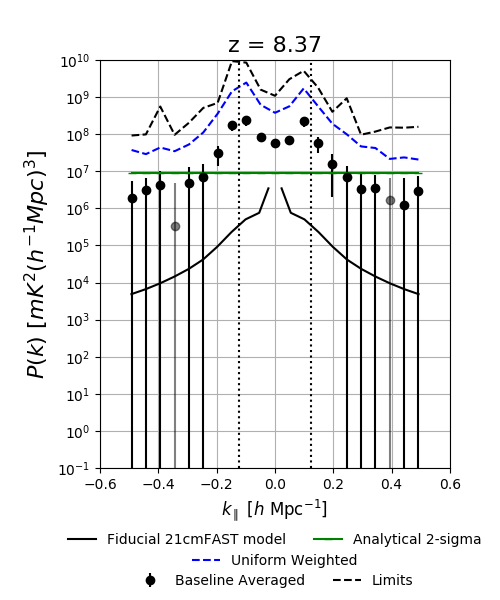
\includegraphics[width=7.5cm]{plots/pspec_95_pk.png} }}%
%    \qquad
%    \subfloat[]{{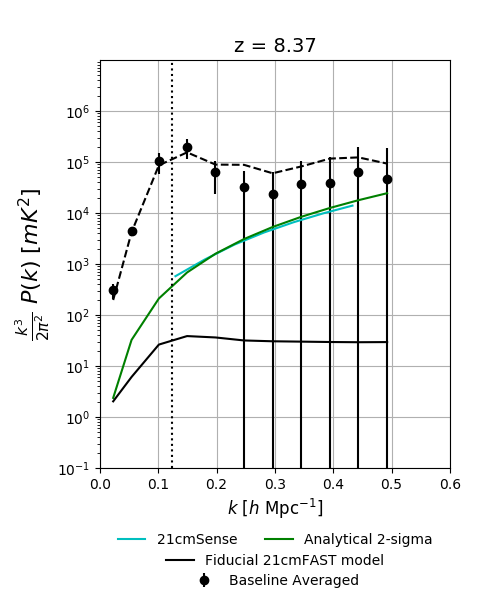
\includegraphics[width=7.5cm]{plots/pspec_95.png} }}%
%    \caption{Power spectrum results at $z=8.37$ shown in (a) $P(k)$ and (b) $\Delta^{2}$
%             using 135 days of PAPER 64 data. For both plots, the pre-signal
%             loss power spectrum estimate is shown with the black points and $2\sigma$
%             error bars. The post-signal loss power spectrum (black dashed curve) shows the 2$\sigma$ upper limit.
%             The uniformly weighted power spectrum (using $\widehat{\textbf{C}}_{x}=\textbf{I}$), is shown as the blue
%             dashed line and does not incur any signal loss by construction.
%             The dotted vertical lines at $k=0.06\hMpci$ show the bounds of the delay filter (or the horizon limit).
%             The analytical (green) 2$\sigma$ noise power spectra assume $T_{rx}=144K$. A fiducial
%             model of the 21cm power spectrum from 21cmFast is shown as the solid black line.}
%    \label{fig:updated_pspec}%
%\end{figure}

%\begin{figure}\centering
%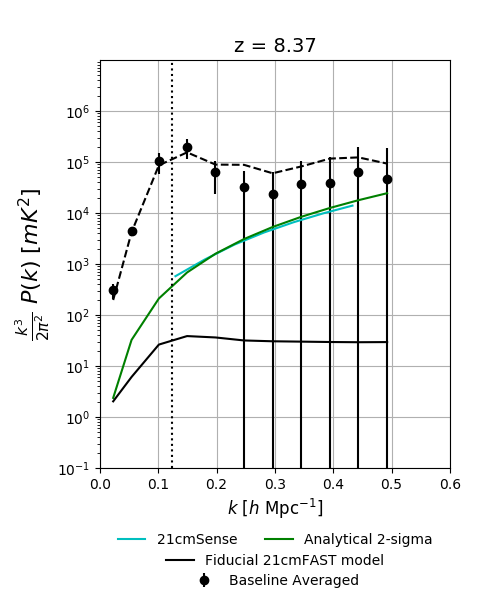
\includegraphics[width=\columnwidth, height=4in]{plots/pspec_95.png}
%%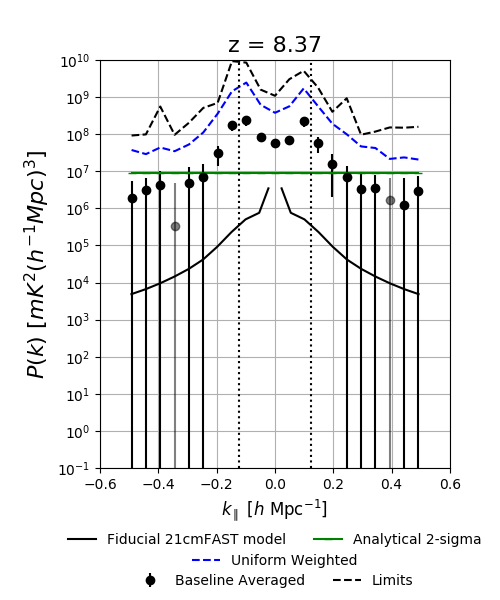
\includegraphics[width=\columnwidth]{plots/pspec_95_pk.png}
%\caption{}
%\label{fig:updataed_pspec}
%\end{figure}
%\clearpage
\nocite{*}
\bibliographystyle{apj}
\bibliography{erratum_biblio}

\end{document}

